\documentclass[11pt]{article}
\usepackage[margin=1in]{geometry}

\usepackage{amssymb}
\usepackage{spalign}
\usepackage{amsmath}
\usepackage{float}
\usepackage{graphicx}
\usepackage[pdfusetitle,
    colorlinks=true,
    linkcolor=red
]{hyperref}

\usepackage[parfill]{parskip}

\title{Vel-Norm Problem Followup}
\author{Sidharth Baskaran}
\date{July 4, 2021}

\begin{document}
% -------------------------------------

\maketitle

\section{Simplifying expression for \texorpdfstring{$w_p(\phi)$}{}}

The sine function is a phase shift of the cosine function, so 
\begin{equation}
    \sin(2k)=\sin(2\phi+\pi/2)=\cos(2\phi).
\end{equation}
It is also given that
\begin{equation}
    2\sin^2(2k)=1-\cos(2k).
\end{equation}
Because $\cos(2k)=-\sin(2\phi)$ by a similar argument, 
\begin{equation}
    2\sin^2(2k)=1+\sin(2\phi).
\end{equation}
Finally
\begin{align}
    w_p(\phi)&=\frac{1}{\underbrace{\sin(2\phi+\pi/2)}_{\cos(2\phi)}}[1\underbrace{-\frac{a_Tr_0^2}{\mu}}_{-\frac{4}{\beta^2(3\pi+8)}}(3\phi+2)]+\frac{2}{\beta^2(3\pi+8)}\underbrace{(2\sin^2(\phi+\pi/4)+3)}_{\sin(2\phi)+4}\\
    &=\frac{1}{\cos(2\phi)}\left[1-\frac{4}{\beta^2(3\pi+8)}(3\phi+2)\right]+\frac{2}{\beta^2(3\pi+8)}(\sin(2\phi)+4)
\end{align}

\section{Numerical evaluation of \texorpdfstring{$y(\phi_m)=0$}{}}

To evaluate $y_p(\phi)=0$, we first define \verb|phi = (1:1:1000)*pi/4/1000|. 
Using this vector to formulate \verb|y_p(Beta)|, where \verb|Beta| is a variable constant, we have a vector of length 1000 representing $y_p(\phi)$.
Note that

\begin{equation}
    y_p(\phi)=\frac{\sqrt{\varphi(\phi)}}{\beta^2(3\pi+8)\sin(2\phi+pi/2)}\sqrt{\frac{\mu}{r_0}}\cot(\phi+\pi/4)
\end{equation}

This implies that $\sin(2\phi+\pi/2)\neq 0$, and further that $y_p$ is only defined for $\varphi(\phi)\geq 0$. Thus, the vector \verb|y_p(Beta)| must be shortened to reflect this and exclude complex numbers.
From calculations, we find that the real representation of $y_p$ is \verb|y_p(Beta)(1:548)| using $a_T=0.2,r_0=1,\mu=1$ with $\beta\approx 1.07$.
To find the section of this vector that is $\in \mathbb{R}$, we have called a function \verb|realBreakpoint(vector)| in Figure \ref{loop1}.
Sorting this vector and determining the corresponding $\phi_m$ solves the problem, where we expect \verb|y_minValue = 0| and \verb|phi_m| to be the corresponding value of $\phi$:

\begin{verbatim}
    [y_values index_vector] = sort(y_p(Beta)(1:548));
    y_minValue = y_values(1);
    phi_m = index_vector(1);
\end{verbatim}

This approach can be extended for a changing parameter $\beta$. 
Since $\delta=\frac{1}{\beta^2}\in (0.001,1)$, $\beta=\sqrt{\frac{1}{\delta}}\in (1,\sqrt{1000})$.
In Octave/MATLAB, we can implement it as

\begin{verbatim}
    delta = (1:1:1000)/1000;
    Beta_vec = sqrt(1./delta);
\end{verbatim}

Mathematically, we say that 
\begin{equation}
\vec\beta=\begin{bmatrix}\beta_1\\\vdots\\\beta_n\end{bmatrix}\text{ and }\vec{\delta}=\begin{bmatrix}1/\beta_1^2\\\vdots\\1/\beta_n^2\end{bmatrix}
\label{paravectors}
\end{equation}
where we choose $n=1000$.
Thus, by iterating through the values of \verb|Beta_vec|, we can generate a corresponding vector \verb|phi_m1| to represent how $\phi_m$ changes with respect to it:

\begin{figure}[H]
    \begin{verbatim}
        phi_m1 = zeros(1,n);
        w_1 = zeros(1,n);
        w_min = zeros(1,n);
        y_0 = zeros(1,n);
    
        for i = 1:n
            y_real = y_p(Beta_vec(i))(1:realBreakpoint(y_p(Beta_vec(i))));
            [yvals idx] = sort(y_real);
            if (length(idx) > 1)
                w_1(i) = w_p(Beta_vec(i))(idx(2));
                phi_m1(i) = phi(idx(2));
                y_0(i) = yvals(2);
            endif
        end
    \end{verbatim}
    \caption{Numerically finding $\vec{\phi_m}$ over $\vec{\delta}$}\label{loop1}
\end{figure}

In Figure \ref{loop1} above, the vector \verb|y_0| is updated with the value $y_p(\phi_{m,i})$ in each iteration
for each value of $\beta$, and is expected to be 0. The vector \verb|w_1| is updated with $w_p(\phi_{m,i})$, which is expected to be unity. As was done with \verb|y_p(Beta)|, 
we have defined a vector \verb|w_p(Beta)| to represent $w_p(\phi)$ where \verb|Beta| is a constant that can be varied.
Thus, we should expect $w_p(\vec\phi_m)=\vec{1}$, $y_p(\vec\phi_m)=\vec{0}\in \mathbb{R}^n$, and the existence of $\vec\phi_m=\begin{bmatrix}\phi_{m,1}\\\vdots\\\phi_{m,n}\end{bmatrix}\in \mathbb{R}^n$ at the end of the loop.
The second index of \verb|y_p(Beta_vec(i)| is accessed to find $\phi_{m,i}$ within the loop because $\phi=0$ always satisfies $y_p(\phi)=0$, and we want to find the second such value.
The conditional check is to account for cases where the domain of $y_p(\phi)\in \mathbb{R}$ is very small (i.e. \verb|length(y_p(Beta_vec(i))| is 1), so we are only able to find $\phi_{m,i}=0\implies y(\phi_m)=0$.

The results of $phi_m$ vs. $\delta$ are expressed in Figure \ref{yminplot} below. $y_p(\phi_m)\approx 0$ and $w_p(\phi_m)\approx 1$ within numerical error, which verifies the validity of these results.

\begin{figure}[H]
    \centering
    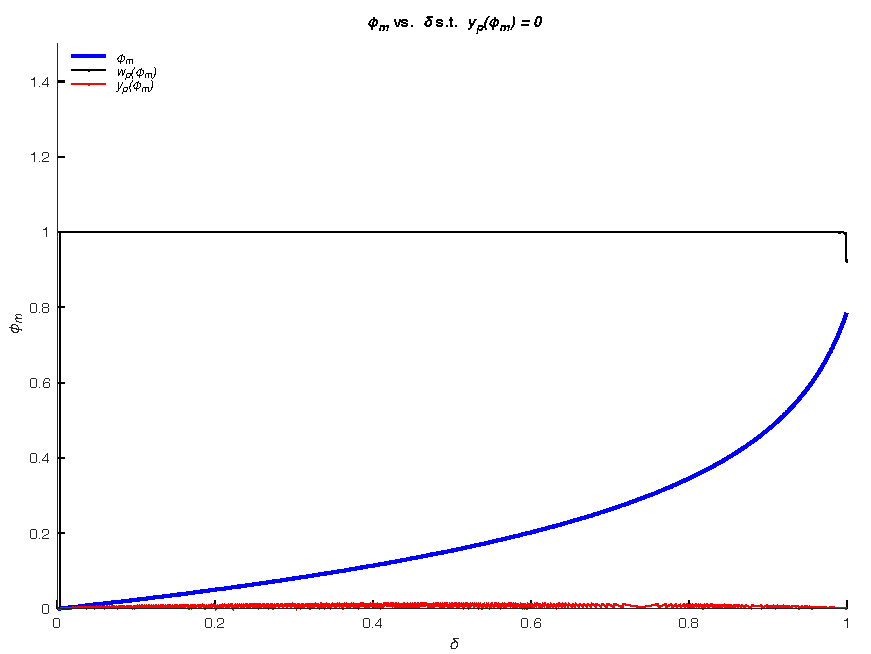
\includegraphics{plots/phi_delta_y.pdf}
    \caption{A plot of these results}\label{yminplot}
\end{figure}

\section{Numerical minimization of \texorpdfstring{$w_p(\phi)$}{}}

We use a similar approach as before to minimize $w_p(\phi)$ numerically. 
In Figure \ref{loop1}, \verb|w_1(i)| was updated
to reflect the value of $w_p(\phi_{m,i})$ where $\phi=\phi_{m,i}$ minimized $y_p(\phi)$ for corresponding values of $\beta_i,\delta_i$
from Eq. \ref{paravectors}. The following code defines a vector \verb|phi_m2| of length $n=1000$ and populates it with the value of $\phi_{m,i}$ that minimizes $w_p(\phi)$ for $\beta_i$.
The corresponding minimum values are stored in another vector \verb|w_min|. Note that the first index of the sorted vector \verb|w_vals| is accessed, since we are looking for the absolute minimum.

\begin{figure}[H]
    \begin{verbatim}
        phi_m2 = zeros(1,n);
        w_min = zeros(1,n);
        for i = 1:n
            [w_vals idx] = sort(w_p(Beta_vec(i)));
            phi_m2(i) = phi(idx(1));
            w_min(i) = w_vals(1);
        end
    \end{verbatim}
    \caption{Iteratively finding $\vec\phi_m$ for $\mathrm{min}(w_p(\phi))$ for various $\beta$}
\end{figure}

Figure \ref{wminplot} below, showing $\phi_m$ (representing \verb|phi_m2|) vs. $\delta$, summarizes these results.

\begin{figure}[H]
    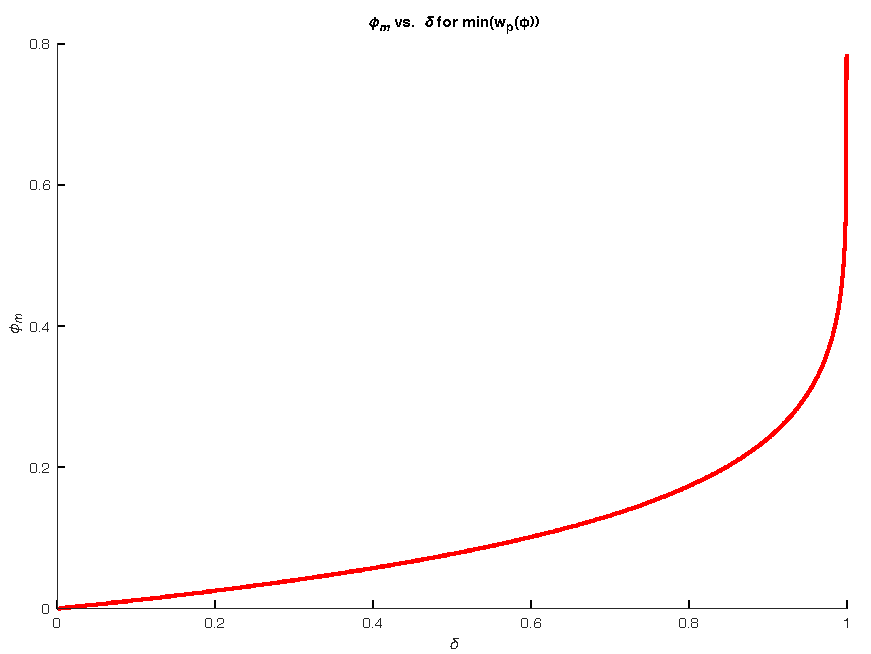
\includegraphics{plots/phi_delta_min.pdf}
    \caption{Values of $\phi_m$ that minimize $w_p(\phi)$ for various $\beta$}\label{wminplot}
\end{figure}

% -------------------------------------
\end{document}